% !TeX root = ../main.tex

\chapter{Evaluation}\label{chapter:Evaluation}

In this chapter, we will first show what our methodology for experimentation was, the reasoning behind each experiment, their value and contribution towards this thesis's goal, and how we went about doing each one. Secondly, we will show, and analyze all the results of said experiments.

\section{Experiments}

The experiments shown in this thesis have been done using our own developed software, shown in chapter 3, and the specifications of the computer used to develop, run, and maintain the software are:

\begin{itemize}
	\item OS: Ubuntu 16.04
	\item CPU: Intel i7 4790k @ 4.6Ghz
	\item RAM: 16GB 1600Mhz
	\item GPU: NVIDIA GTX 1080
\end{itemize}

And though the specifications of this computer are well above what was needed to both, develop and run our experiments, we can say with certainty that any computer with similar specifications can replicate anything shown in this chapter with ease.

\subsection{Docker container setup}

We have mentioned previously the use of MACKE but never touched on the topic of its setup. MACKE being a wrapper around KLEE, requires a full installation of first, a specific version of KLEE, which in and of itself can be a lengthy process. Furthermore, some programs need to be installed in a specific order -- not all -- and if a step is omitted or disregarded, KLEE and MACKE are sure to not run properly, be erratic, or flat-out not work.

Seeing this as a problem, and knowing that our experiments needed the utmost precision, and sometimes required a bit of experimentation with some of the programs involved, we knew we had to create an environment that could be shared with us, that was confirmed to be working fine, that was disposable, yet upgradable. To this end, we developed a Docker \parencite{docker} image, which has MACKE completely configured, and ready to be executed. The image is also disposable and can be run and discarded as many times as needed. The image can be downloaded by doing:

\begin{lstlisting}[language=bash]
$ docker pull ricardonales/make:0.6
\end{lstlisting}

And to run the image, and work with it:

\begin{lstlisting}[language=bash]
$ docker run -ti ricardonales/macke:0.6 bash
\end{lstlisting}

Then we need to start Python virtual environment where MACKE is available, and in order to do this we need to run the following command (it is worth noting that the container only has the root user, so the next command needs to be written "as is"):

\begin{lstlisting}[language=bash]
# source ~/build/macke/.venv/bin/activate
\end{lstlisting}

After doing this MACKE will be available by running "macke" as shown in Figure 4.1.

\begin{figure}[H]
	\caption{MACKE running on container}
	\centering
	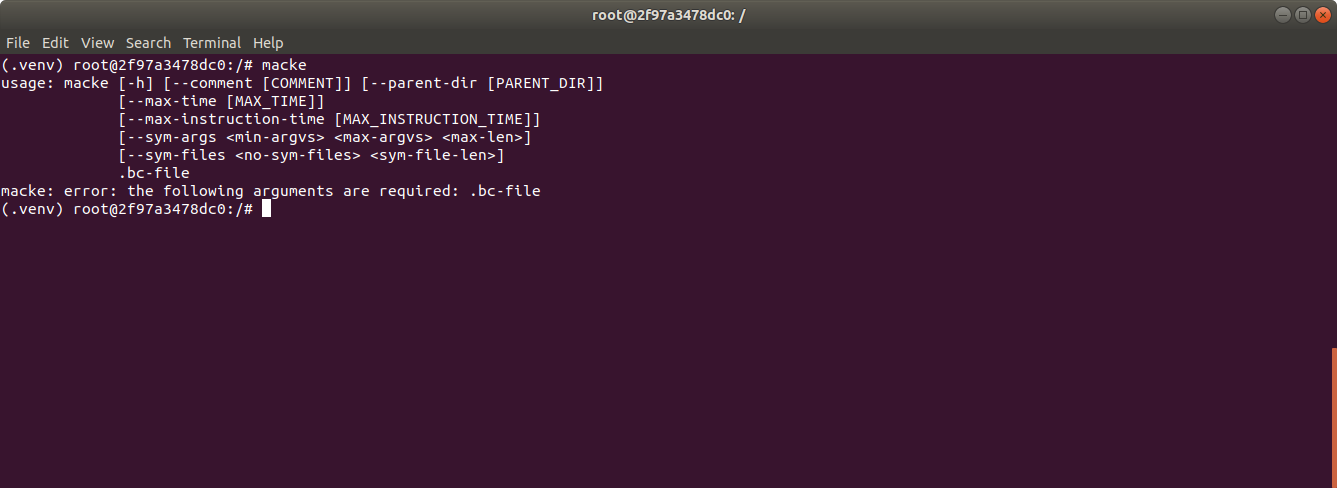
\includegraphics[width=1.0\textwidth]{macke_container}
\end{figure}


\subsection{Pre-processing the data}

In order to be able to run programs through MACKE we require to have their bitcode files generated by compiling them with LLVM, in order to do this, using our pre-configured container with all tools needed, we need to run the programs through "make+llvm", to do so we did the following:
\\

Enter the MACKE container and run the following command to enter the Python virtual environment containing make+llvm:

\begin{lstlisting}[language=bash]
# source ~/build/MakeAdditions/.venv/bin/activate
\end{lstlisting}

This will allow the program make+llvm \parencite{thomasThesis}. The next step needed is to go to our program and run its "configure" file so that it generates its Makefile, which is needed by make+llvm.

The next thing we did was run make+llvm on the Makefile by running:

\begin{lstlisting}[language=bash]
# make+llvm Makefile
\end{lstlisting}

This process might take some time, since it will first build the required files from the Makefile, and then immediately run llvm on it. This process will generate, if successful, all binary files needed.

Alternatively, one can run LLVM directly on a specific $c$ or $cpp$ file by doing the following:

\begin{lstlisting}[language=bash]
# clang -I <LIBRARIES_FOLDER> -emit-llvm -c -g <FILE>.c
\end{lstlisting}

We point out that <LIBRARIES\_FOLDER> must include the path (relative or absolute). By doing this, we can also generate the bitcode of a specific file.

This is al the pre-processing needed in order to be able to work with the programs. It is extremely important to point out that not all programs will compile with make+llvm, and that sometimes there will be the need to isolate files, and run clang or clang++ directly on them.

\subsection{Runnig MACKE on programs}

Once all the bitcode files have been extracted for all programs, we are able to run MACKE on them, and with the container already pre-configured and with a proper MACKE installation, we can say with certainty that running the following commands will lead to the desired outcome:

\begin{lstlisting}[language=bash]
# macke <PROGRAM>.bc
\end{lstlisting}

With that, MACKE will run the program and run the composite symbolic execution, which can take up to hours depending on how big the program analyzed is. The result of running MACKE over rzip.bc is shown in Figure 4.2.

\begin{figure}[H]
	\caption{Running MACKE on rzip}
	\centering
	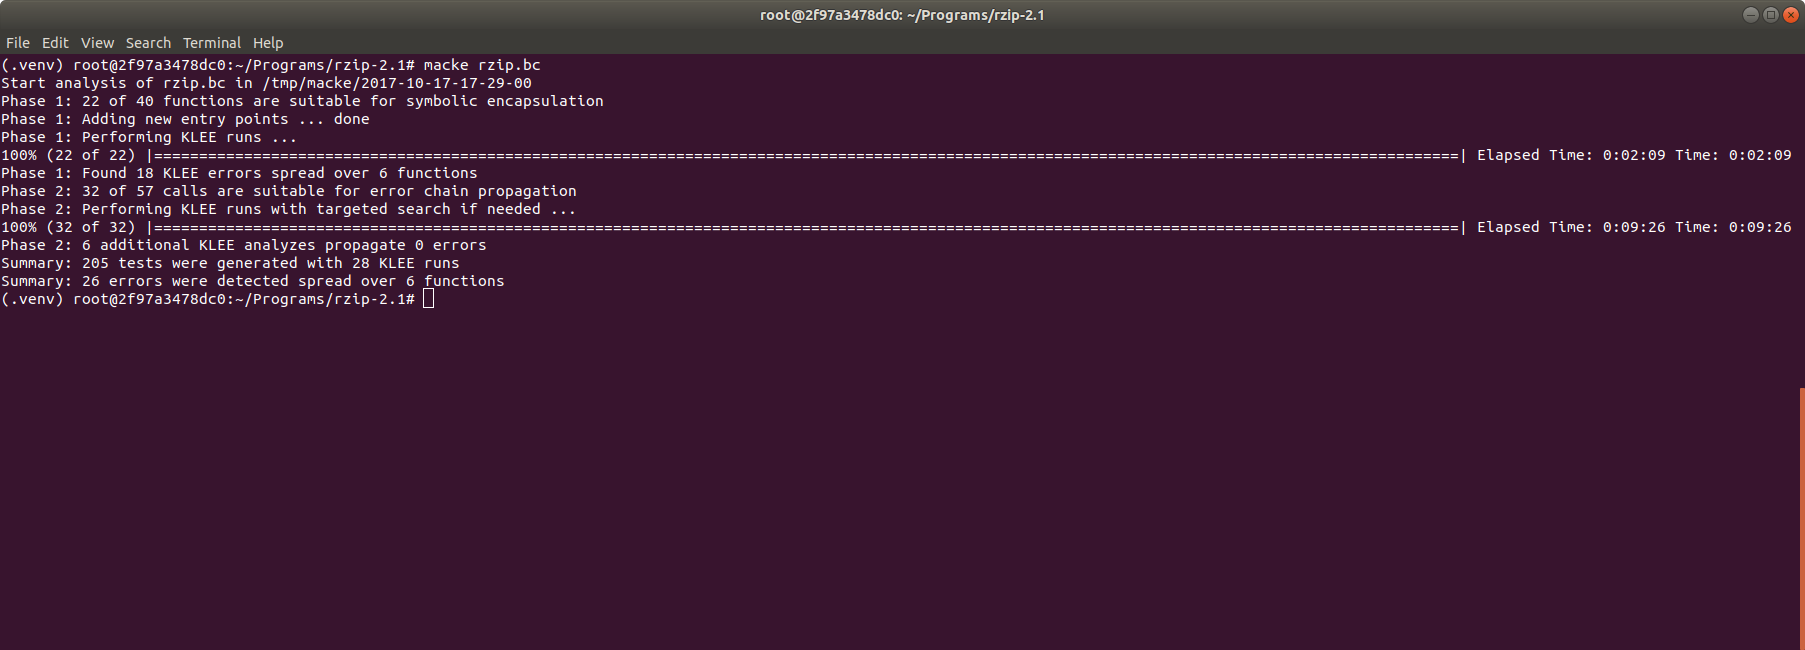
\includegraphics[width=1.0\textwidth]{macke_on_rzip}
\end{figure}

As we can see MACKE found 26 vulnerabilities spread across 6 functions. To see this data one must go to the results folder, which is found under "/tmp/macke/macke-last", or if it is not the latest run of MACKE, it will be under "/tmp/macke/DATETIME\_WHEN\_RUN". The file that has the results information is klee.json, which we can read with either with a simple :

\begin{lstlisting}[language=bash]
# cat klee.json
\end{lstlisting}

Or by running:

\begin{lstlisting}[language=bash]
# jq . klee.json
\end{lstlisting}

We used this last option since the result is much more readable and structured. The results of rzip can be seen in Figure 4.3.

\begin{figure}[H]
	\caption{MACKE rzip's results}
	\centering
	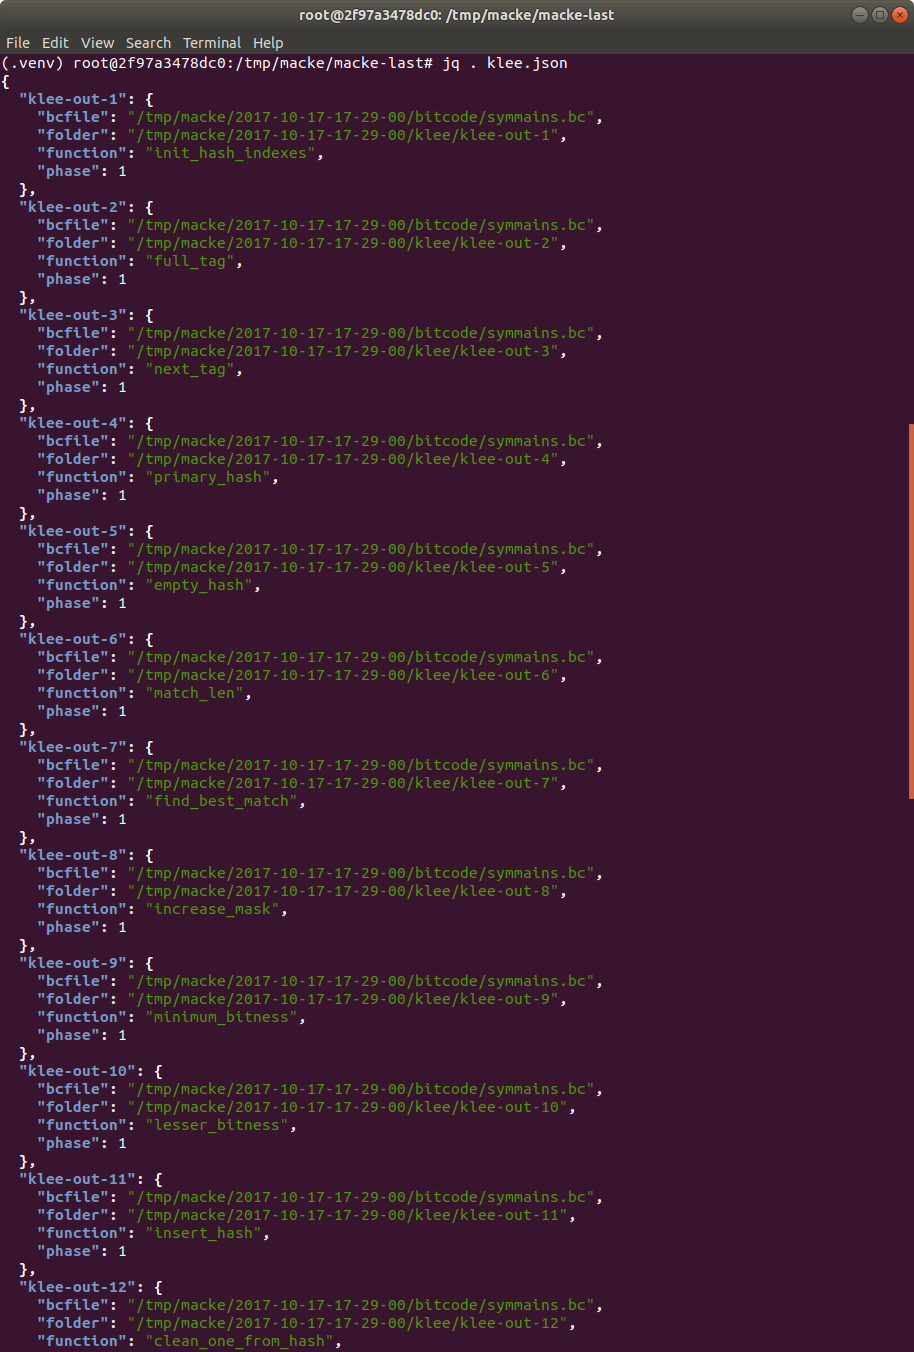
\includegraphics[width=0.9\textwidth]{macke_rzip_results}
\end{figure}

\subsection{CVSS score assignment}

Using the NVD database to use reliable data, that met the criteria detailed in chapter 3, we created a compilation of the CVSS3 scores of the functions with vulnerabilities. To do this, we first searched through the NVD provided JSON files which include all vulnerabilities found in a structured way. In said files, we searched for the "CVE Dictionary Entry" as NVD calls it \parencite{nvd} and compiled all of them in a new structure, which can be seen in Figure 4.4.

\begin{figure}[H]
	\caption{CVSS3 Scores File}
	\centering
	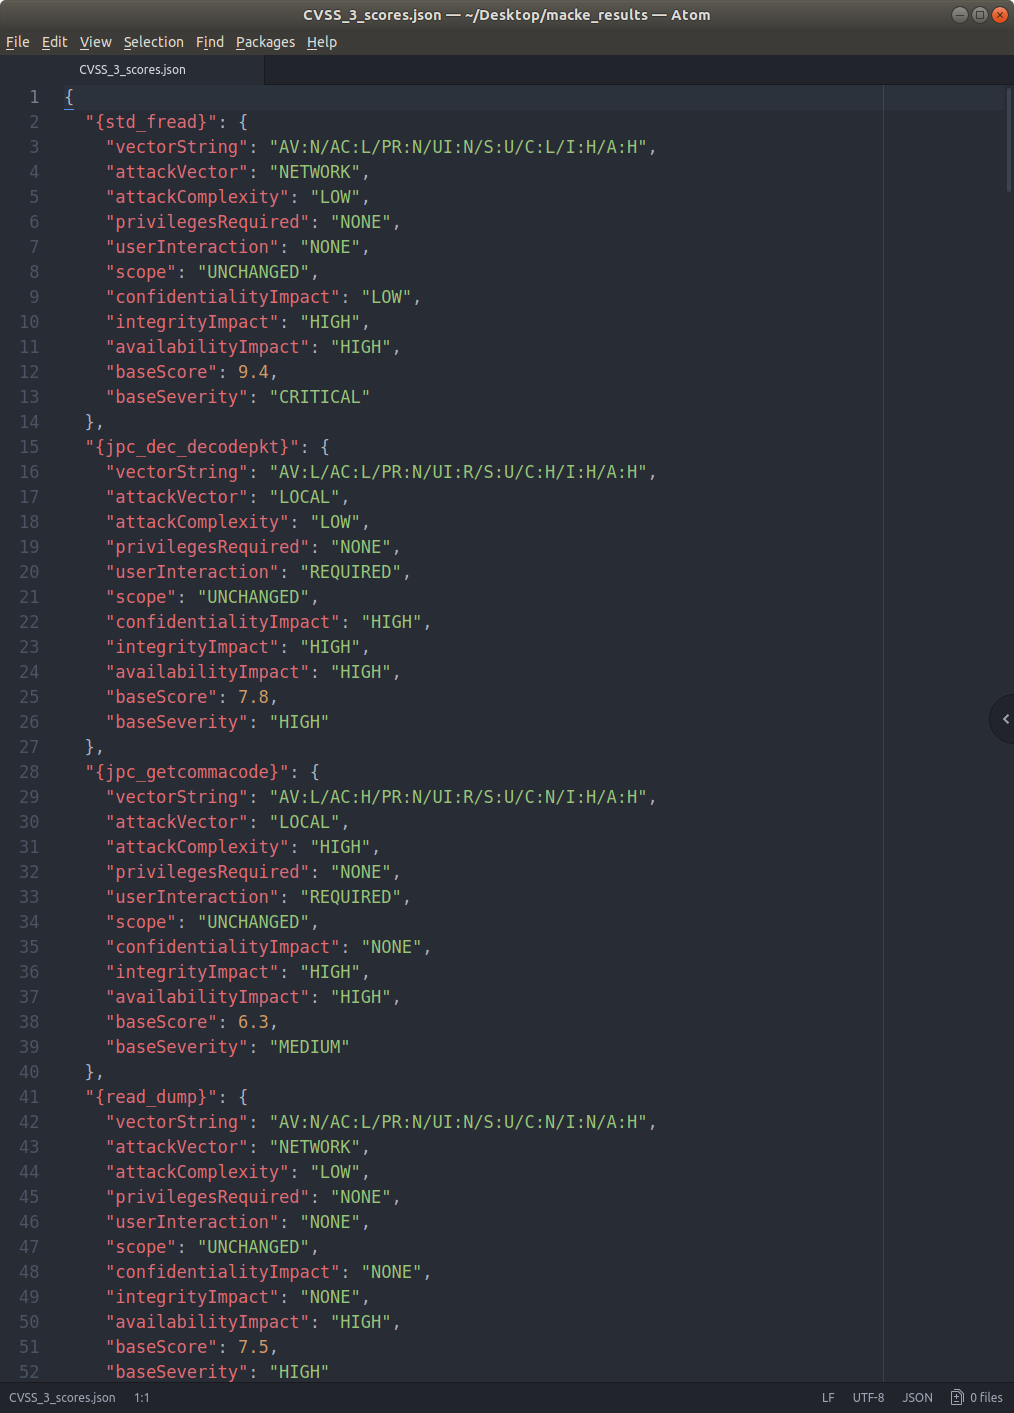
\includegraphics[width=0.9\textwidth]{cvss_file}
\end{figure}

This scores would allow us to map them to the vulnerabilities found through MACKE. There was a problem with this solution though: our pool of base scores was too low, 24 to be precise.

Knowing this we set out to manually extract the base scores of the rest of vulnerabilities that were buffer overflow related. This procedure was lengthy and not straightforward and showed us how subjective assessing some of the base scores can be. Furthermore, by looking at the procedure manually we were able to see that there were patterns, yet they could not be proven until we ran tests with the node attributes we had selected as the impact factors of the CVSS3 scores.

We were able to collect 23 more samples, which in total allowed us to get a total of 47 CVSS3 scores which we were certain had been thoroughly analyzed and could be reliably used for learning purposes without having noisy data.

\subsection{Getting Call Graphs and Node Attributes}

The data that we had from all programs, after running LLVM on them was a bitcode file, but with this, we still needed to extract the dot -- which has the call graph information -- from the bitcode. This has already been thoroughly explained in chapter 3.

Furthermore, and as mentioned as well in the aforementioned chapter, we were able to remove all redundant edges from the original callgraph, therefore allowing us to make a proper analysis of the call graphs.

The pre-processing of the data was mainly running all programs through our Python node\_attributes program, which generates a file that has the same name of the source dot file, with "\_node\_attributes.json" appended to it. This file contains all nodes, with their respective node attributes. In the case that CVSS3 scores were available from NVD, or the manually extracted CVSS3 --explained to detail in the next subsection -- scores we extracted. This is shown in Figure  4.3.

\begin{figure}[H]
	\caption{Pre-processed Data}
	\centering
	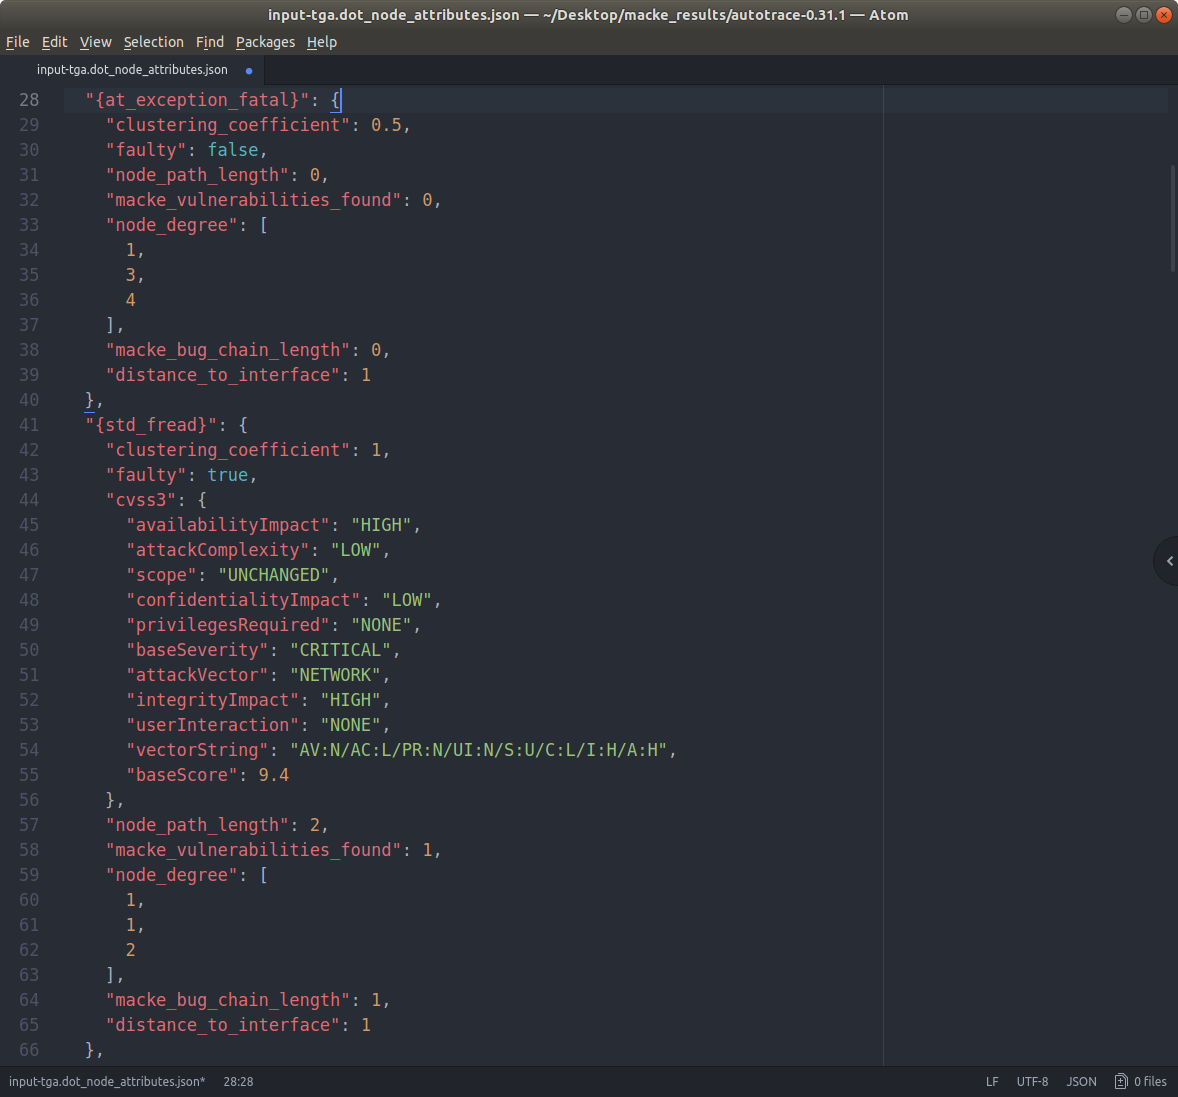
\includegraphics[width=1.0\textwidth]{preprocessed_data}
\end{figure}

This file does not contain callgraph data, it is only the node attributes data, and if we had available CVSS3 data, from our compilation of base scores.

\subsection{Learning Setup}

Now that we have a set of node attributes for every single function that is vulnerable, along with all of the CVSS3 scores from both sources, the NVD database and the scores we manually extracted. We will be calling $X$ all of the node attributes from all of our vulnerable functions which have a CVSS3 score. And $y$ will be all of the resulting classes for a specific base score metric from CVSS3, for example, $y_AV$ would be the collection of all categories found for the "Attack Vector". The same was done for all different base score metrics. In order learn from this data our algorithm needs to use our set of $X$ against each set $y$. As a result of this learning we would have a model that could classify an unseen sample that only has node attributes, yet no CVSS3 scores.

In other words, and to better exemplify this, if we think of all the gathered node attributes of functions for which we had CVSS3 scores available, and stored them in an array called $X$. Each index of the array holds the node attributes of each different function. Now, we know that these node attributes have a relation to a CVSS3 score that was given, which is divided into several base score metric. These metrics for each function we will separate, and generate different arrays called $y$ of its respective base score metric, so for example, $y_AV$ would hold all resulting Attack Vector scores for all functions, and the same would be done for the rest of the base score metrics.

We have shown both parts needed in order for us to be able to use a learning algorithm:

\begin{enumerate}
	\item The $X$ is the node attributes found on a per-node basis.
	\item We have several $y$, one for every CVSS3 base score. 
\end{enumerate}

In order to implement, and test different learning algorithms we chose to use SciKit \parencite{scikit}, which is one of the most widely used Python libraries in the world for machine learning. With this library, we would be able to test two different classifier algorithms and see how they behaved.

\subsubsection{Random Forest and Naive Bayes}

We decided to use these two classifiers since both have been shown to be robust classifiers, though we had to compare their theoretical efficiency. Following is a list of pros/cons of each classifier.
\\\\
Random Forests:
\begin{itemize}
	\item + It is robust against overfitting
	\item + It gives better results with the increasing number of examples
	\item + It might be used for clustering, statistical inference and feature selection as well
	\item + Works well with numerical, categorical data
	\item - Slower to train
	\item - Need to be set well its randomization parameters. (Selection of nodes, number of trees, randomization of instance variables)
	\item - Some objections for it overfitting
\end{itemize}
Naive Bayes:
\begin{itemize}
	\item + Easy to trains and understand the results
	\item + It has different extensions for different needs
	\item + Its model is smaller than the random forests since you need to keep all the trees in memory
	\item + Promising results for textual tasks
	\item - Based on naive assumptions that are not generally concordant with the data
	\item - It is really fragile to overfitting without any regularization assumption
\end{itemize}

These benefits and drawbacks of each one give us an outlook of how results will look, though only through experimentation would we be able to see if these applied to our dataset.

\subsubsection{Split dataset}

We have already mentioned that we divided our data into $X$ and $y$ as per usual in all machine learning procedures \parencite{scikit}. The next step was to select how we would be fitting our models, according to our limited dataset of only 47 entries (of vulnerable functions with their respective CVSS3 score).

To test this we decided to use 4 folds, using K-Fold cross-validation, in which the original sample is randomly partitioned into k equal sized subsamples. Of the k subsamples, a single subsample is retained as the validation data for testing the model, and the remaining k - 1 subsamples are used as training data. The cross-validation process is then repeated k time because that would allow us to find four possible models out of our data, and compare each other. Out of these four models, we would then be able to find the best one and select it from all of them and use this as our final model.

\subsection{Front-end implementation}

One of the crucial parts of our thesis is the front-end since it is the point where users can finally interact with everything else that has been developed. Right from the beginning, we knew our framework would need to fulfill the following requirements:

\begin{enumerate}
	\item Be a web application that can be accessed remotely
	\item Have a simple user interface and good user experience
	\item Implement a way for users to let us know how we could improve
\end{enumerate}

What we decided to develop was a Client-Server application that uses HTTPS as a secure link between the two when passing requests and responses. The application stack looks as follows:

\begin{itemize}
	\item Back-end: NodeJS using Express as the server API 
	\item Front-end: ReactJS using server-side rendering
\end{itemize}

What we mean by server-side rendering, is that NodeJS being able to render JS code, it allows for faster loading times, since the browser does not need to render the initially received JS code, since it has already been rendered to HTML. This speeds-up the process in slow computers, and also makes the backend structure more robust since we are able to fine-grain handle requests, instead of just sending the entire ReactJS bundle along with a dummy HTML page. All this code can be analyzed under \parencite{ricardo} and follows the normal structure of SSR ReactJS applications.

\begin{figure}[H]
	\caption{Front-end tutorial page}
	\centering
	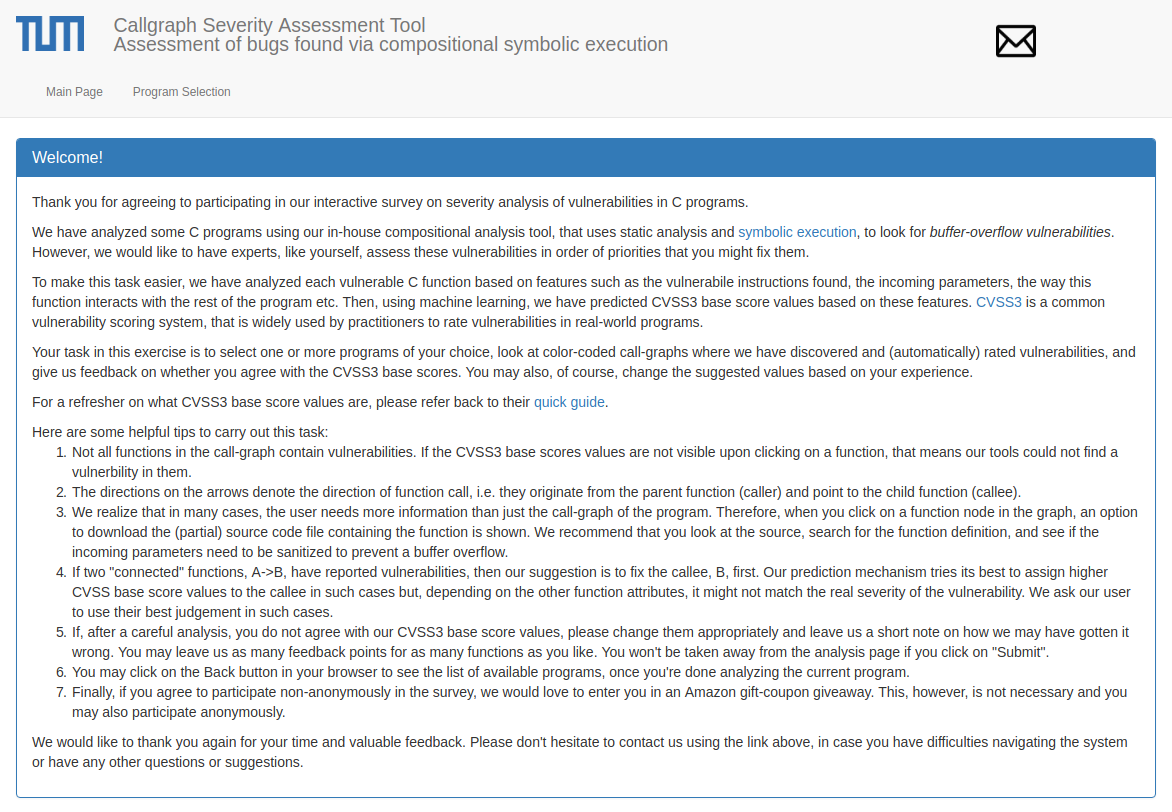
\includegraphics[width=1.0\textwidth]{explanation_frontend}
\end{figure}

First, we added a "Tutorial" page where we explain to the user what they are about to do, what they can expect, and what we are expecting of them as well. This can be seen in Figure 4.6.

Second, we show the users what they should do in a step by step manner. This part is very thorough so that in case a user happens to get stuck, they have always these instructions to fall back on. This can be seen in Figure 4.7.

\begin{figure}[H]
	\caption{Front-end instructions}
	\centering
	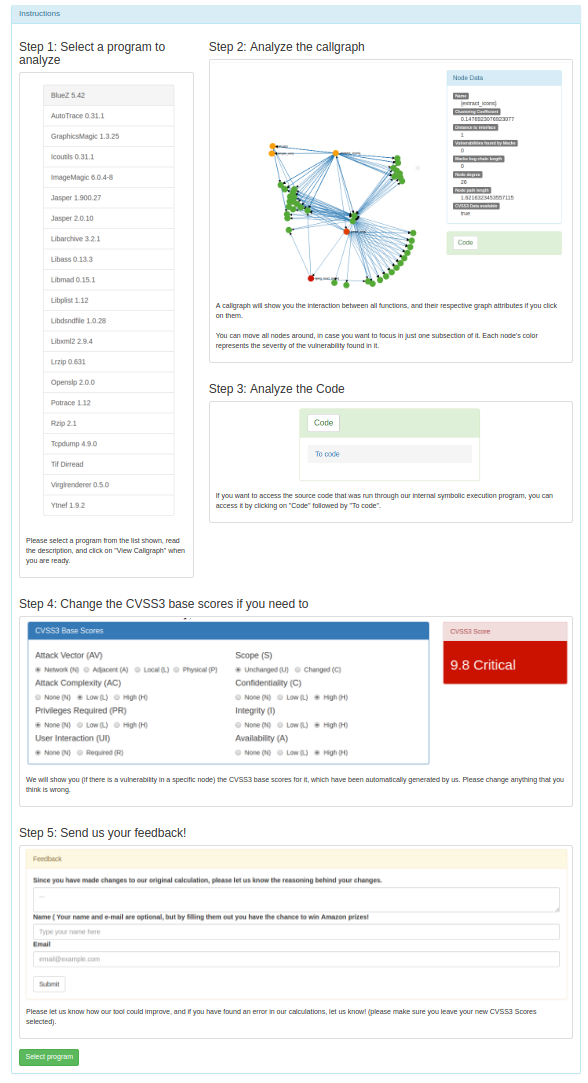
\includegraphics[width=0.6\textwidth]{instructions}
\end{figure}

When the user clicks either on the navigation bar on "Program Selection" or on the green button under our instructions "Select Program" they are taken to the next step, which consists of a selection of the program that they would like to analyze out of all the programs mentioned in 3.3.1. 

\begin{figure}[H]
	\caption{Front-end program selection}
	\centering
	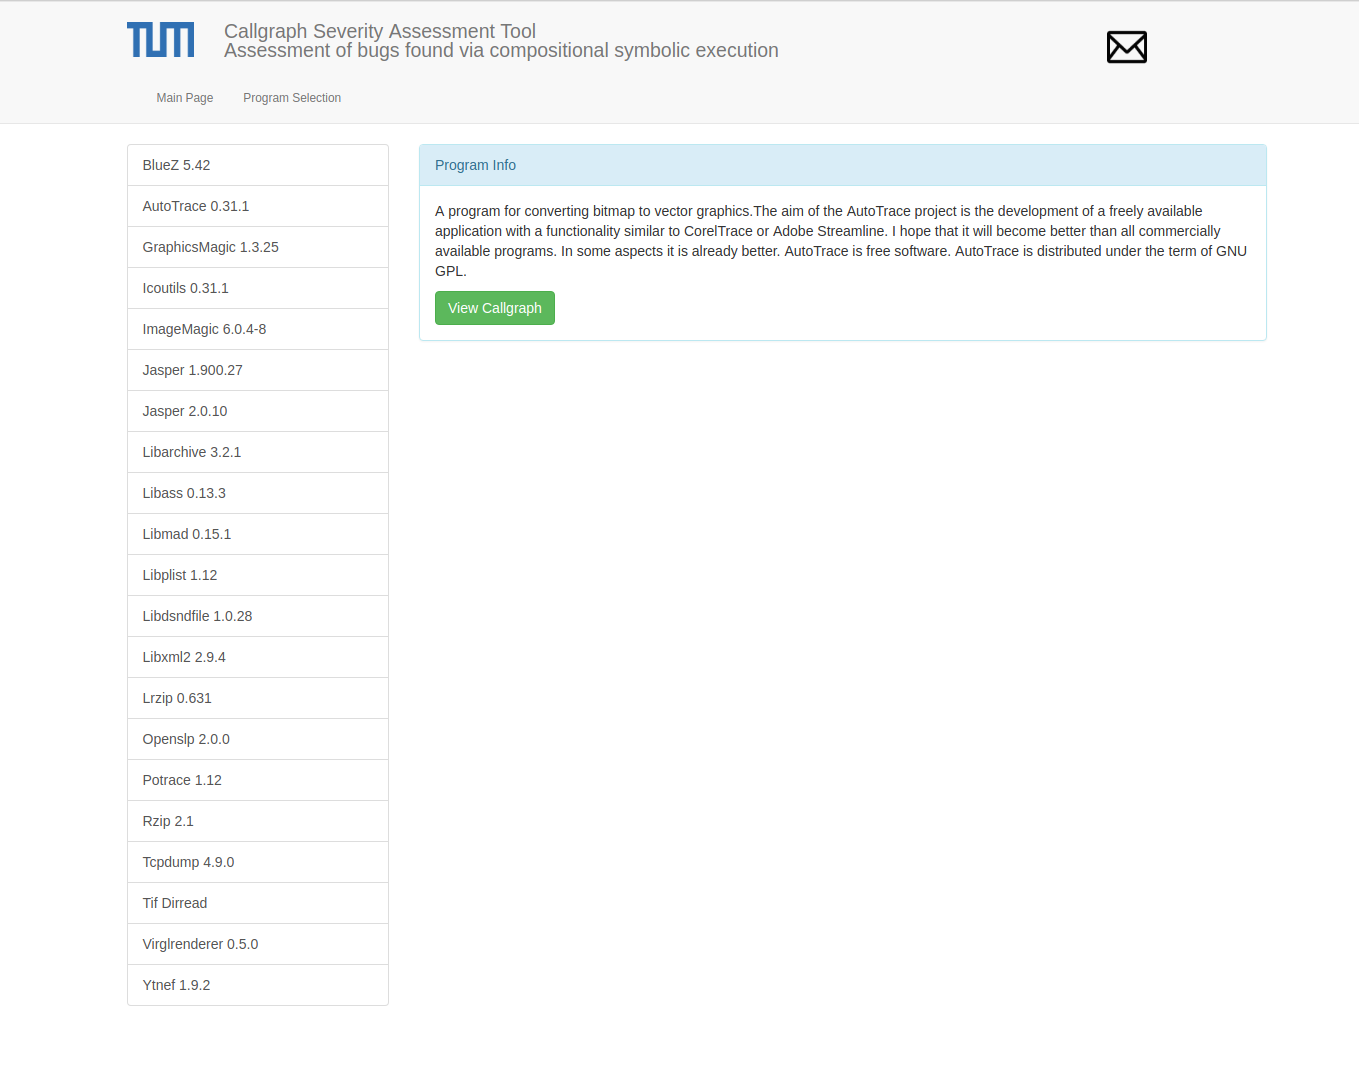
\includegraphics[width=1.0\textwidth]{program_selection}
\end{figure}

Once the user clicks on "View Callgraph" he will be shown the view shown in Figure 4.9. It includes the Callgraph on the top part, which is fully interactable, a reference on the color coding used on nodes depending on their CVSS3 severity \parencite{cvss3}. If the user clicks on "Code" a menu is expanded that allows the download of the source code used to get the Callgraph shown. The "Node Attributes" button is also collapsed and needs to be clicked on in order to expand all node attributes of the currently selected node. The bottom part shows the CVSS3 base scores if they are available. It works in the form of a calculator, identical to official CVSS 3.0 calculator found at \parencite{cvss3} and will show the new severity score as soon as a base score changes. 

\begin{figure}[H]
	\caption{Front-end Callgraph and CVSS3 Scores}
	\centering
	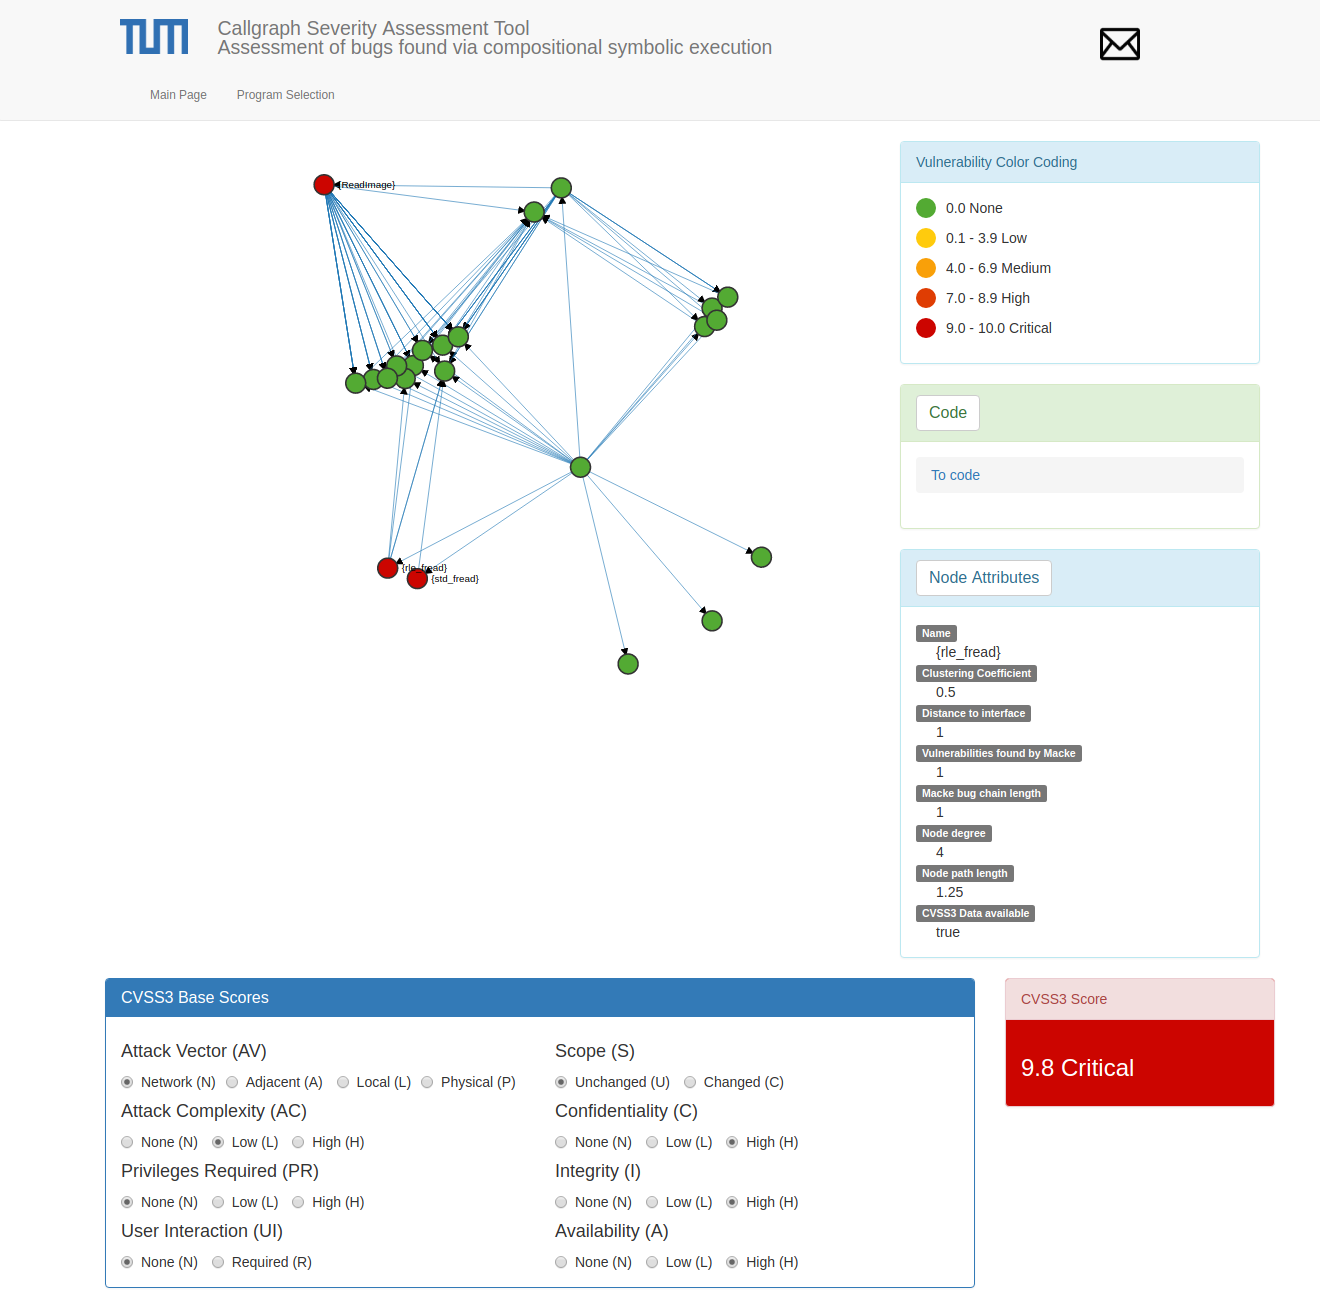
\includegraphics[width=1.0\textwidth]{callgraph_and_cvss}
\end{figure}

By having all of these features we fulfilled what we set out to do in terms of requirements, though we know there is room for improvement, and that we require feedback from professionals, which leads us to the Survey.

\subsection{Survey}

The target group of our framework is professionals in the area of IT Security with experience in C or C++, who could assess the vulnerabilities with the use of CVSS3 manually. There needs to be a way for said professionals to let us know what they think of the results provided by our framework.

Our front-end implementation includes a Survey that allows users to send us their opinion about the framework. A screenshot of the Survey can be seen in Figure 4.6

\begin{figure}[H]
	\caption{Survey}
	\centering
	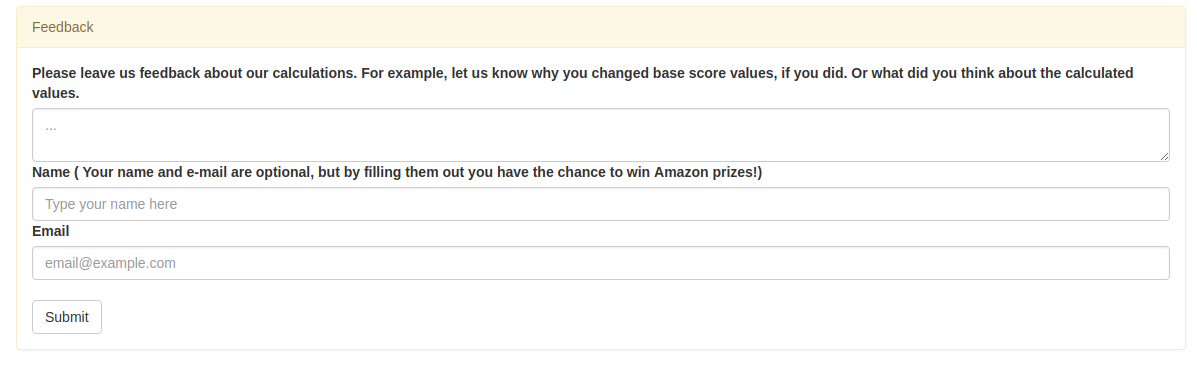
\includegraphics[width=1.0\textwidth]{survey}
\end{figure}

As shown, we leave the user's personal information as optional and focus mainly on their opinion. We incentivize the user to give us their personal information in case we need to get back to them and ask them for further feedback and/or advice on how to improve upon what has already been developed.

\subsection{Including Feedback}

All of the feedback is invaluable to us, the reasoning behind this has to do with the nature of vulnerabilities and CVSS itself. When assessing them, as shown in section 4.1.4, it can sometimes be hard to come up with a score that is not only accurate but free of personal bias. To this end, we have added the previously mentioned Survey. All feedback received will be added as future work for this project, and will shape the project in the long term. Depending completely on the data received from the survey will we know how good our model fares when predicting the base scores of vulnerabilities found through symbolic execution, and if the impact factors selected such as the node attributes either need to be changed or improved.

\section{Results}

In the previous section, we have shown all the requirements and the preparation of the tools needed for our experimentation. In this section, we will show all the results and draw conclusions regarding what the experimental data showed against our hypothesis, and previous assumptions. 

\subsection{MACKE vulnerabilities found}

After running MACKE on all 21 programs listed under section 3.3.1, we were able to find a wide variety of vulnerabilities in across all programs. In the following table we list the results for each program:

\begin{table}[H]
	\centering
	\caption{MACKE vulnerabilities found Part 1}
	\begin{tabular}{ |p{4cm}||p{10cm}|  }
		\hline
		Program & Functions with vulnerabilities\\
		\hline
		BlueZ 5.42   & p\_indent, parse, process\_frames, read\_n, read\_dump, read\_dump \\
		AutoTrace 0.31.1 &   ReadImage, rle\_fread, std\_fread \\
		GraphicsMagic 1.3.25 & MagickArraySize, MagickMalloc, MagickMallocAligned, MagickMallocAlignedArray, MagickMallocArray, MagickMallocCleared, MagickCloneMemory, MagickFree, MagickRealloc, MagickFreeAligned \\
		,    Icoutils 0.31.1    & xfread, read\_png, simple\_vec, png\_read\_mem, extract\_icons \\
		ImageMagic 6.0.4-8    & RegisterRLEImage, ScaleShortToQuantum, IsValidColormapIndex, ScaleCharToQuantum, SetImageProgress, ReadRLEImage, IsRLE, UnregisterRLEImage  \\
		Jasper 1.900.27    & jas\_safe\_size\_mul, jas\_matrix\_destroy, jas\_matrix\_create, jas\_seq2d\_create, jas\_seq2d\_copy, jas\_matrix\_copy, jas\_matrix\_bindsub, jas\_seq2d\_bindsub, jas\_matrix\_cmp, jas\_matrix\_divpow2, jas\_matrix\_clip, jas\_fast32\_asr, jas\_matrix\_asr, jas\_fast32\_asl, jas\_matrix\_asl, jas\_matrix\_resize, jas\_matrix\_setall, jas\_seq2d\_input, jas\_seq2d\_output\\
		Jasper 2.0.10    & jpc\_dec\_lookahead, jpc\_getnumnewpasses, jpc\_getcommacode, jpc\_dec\_decodepkt, jpc\_dec\_decodepkts, jpc\_dec\_pi\_create\\
		Libsarchive 3.2.1    & bsdtar\_expand\_char, safe\_fprintf, yes, set\_chdir, do\_chdir, strip\_components, warn\_strip\_drive\_letter, warn\_strip\_leading\_char, strip\_absolute\_path, edit\_pathname, tar\_i64toa, pathcmp, passphrase\_callback, passphrase\_free, list\_item\_verbose\\
		Libass 0.13.3    & calc\_coeff, ass\_stripe\_unpack\_c, ass\_stripe\_pack\_c, get\_line, copy\_line, shrink\_func, ass\_shrink\_horz\_c, ass\_shrink\_vert\_c, expand\_func, ass\_expand\_horz\_c, ass\_expand\_vert\_c, pre\_blur1\_func, ass\_pre\_blur1\_horz\_c, ass\_pre\_blur1\_vert\_c, pre\_blur2\_func, ass\_pre\_blur2\_horz\_c, ass\_pre\_blur2\_vert\_c, ass\_pre\_blur2\_vert\_c, ass\_pre\_blur3\_horz\_c, ass\_pre\_blur3\_vert\_c, blur\_func, ass\_blur1234\_horz\_c, ass\_blur1234\_vert\_c, ass\_blur1235\_horz\_c, ass\_blur1235\_vert\_c, ass\_blur1246\_horz\_c, ass\_blur1246\_vert\_c, calc\_gauss, coeff\_filter \\
		\hline
	\end{tabular}
\end{table}


\begin{table}[H]
	\centering
	\caption{MACKE vulnerabilities found Part 2}
	\begin{tabular}{ |p{4cm}||p{10cm}|  }
		\hline
		Program & Functions with vulnerabilities\\
		\hline
		Libmad 0.15.1    & III\_imdct\_s, fastsdct, III\_imdct\_l, mad\_layer\_III \\
		Libplist 1.12    & byte\_convert, uint24\_from\_be, float\_byte\_convert, parse\_real\_node, parse\_date\_nodec, parse\_data\_node, parse\_string\_node, plist\_utf16\_to\_utf8, parse\_unicode\_node, parse\_array\_node, parse\_dict\_node, copy\_plist\_data, serialize\_plist, write\_uint, write\_uint, write\_real, is\_ascii\_string, write\_raw\_data, write\_string, write\_string, write\_unicode, write\_data, write\_array, write\_dict, write\_date, write\_uid, plist\_data\_hash\\
		Libdsndfile 1.0.28    & i2les\_array, pcm\_init, sc2s\_array, pcm\_read\_sc2s, sc2i\_array, pcm\_read\_sc2i, sc2f\_array, pcm\_read\_sc2f, sc2d\_array, pcm\_read\_sc2d, uc2s\_array, pcm\_read\_uc2s, uc2s\_array, pcm\_read\_uc2s, uc2i\_array, pcm\_read\_uc2i, uc2f\_array, pcm\_read\_uc2f, uc2d\_array, pcm\_read\_uc2d, ENDSWAP\_16, endswap\_short\_array, pcm\_read\_bes2s, bes2i\_array, pcm\_read\_bes2i, bes2f\_array, pcm\_read\_bes2i, bes2f\_array, pcm\_read\_bes2f, bes2d\_array, pcm\_read\_bes2d, bet2s\_array, pcm\_read\_bet2s, psf\_get\_be24, bet2i\_array, pcm\_read\_bet2i, bet2f\_array, pcm\_read\_bet2f, bet2d\_array\\
		Libxml2 2.9.4    & xmlInitializeDict, \_\_xmlInitializeDict, \_\_xmlRandom, xmlDictCleanup, xmlDictCreate, xmlDictReference, xmlDictCreateSub, xmlDictFree, xmlDictComputeFastKey, xmlDictComputeBigKey, xmlDictAddString, xmlDictGrow, xmlDictLookup, xmlDictExists, xmlDictComputeFastQKey, xmlDictComputeBigQKey, xmlDictAddQString, xmlDictQLookup, xmlDictOwns, xmlDictSize, xmlDictSetLimit, xmlDictGetUsage\\
		Lrzip 0.631    & fatal, init\_mutex, unlock\_mutex, read\_1g,  lock\_mutex, detach\_pthread, print\_stuff \\
		Openslp 2.0.0    & strncasecmp, ishex, hex2bin, SLPNormalizeString, SLPUnescapeInPlace, SLPFoldWhiteSpace, SLPCompareNormalizedString, SLPCompareString, SLPCompareNamingAuth, SLPCompareSrvType, SLPContainsStringList, SLPIntersectStringList,SLPIntersectRemoveStringList, SLPUnionStringList, SLPSubsetStringList. SLPCheckServiceUrlSyntax, SLPCheckAttributeListSyntax \\
		\hline
	\end{tabular}
\end{table}

\begin{table}[H]
	\centering
	\caption{MACKE vulnerabilities found Part 3}
	\begin{tabular}{ |p{4cm}||p{10cm}|  }
		\hline
		Program & Functions with vulnerabilities\\
		\hline
		Potrace 1.12    & fgetc\_ws, readnum, bm\_new, bm\_clear, readbit, bm\_free, bmp\_readint, bmp\_forward, bmp\_pad\_reset, bmp\_pad, bm\_readbody\_bmp, lobit, bm\_writepbm, bm\_print \\
		Rzip 2.1    & write\_buf, write\_u8, write\_u16, write\_u32, open\_stream\_out, read\_buf, read\_u8, read\_u16, read\_u32, open\_stream\_in, seekto, compress\_buf, flush\_buffer, write\_stream, write\_stream, fill\_buffer, read\_stream, close\_stream\_out, close\_stream\_in \\
		Tcpdump 4.9.0    & EXTRACT\_16BITS, EXTRACT\_32BITS, print\_long\_pos\_vector, print\_btp, print\_btp\_body, geonet\_print, GeoNetworking \\
		Tif Firread    & TIFFCheckDirOffset, TIFFReadUInt64, readContigStripsIntoBuffer, TIFFReadDirectoryCheckOrder, TIFFReadDirectoryFindEntry, TIFFReadDirectoryFindFieldInfo \\
		Virglrenderer 0.5.0    & uprcase, is\_digit, is\_alpha\_underscore, is\_digit\_alpha\_underscore, debug\_printf, report\_error, parse\_header, parse\_label, parse\_register\_file\_bracket, parse\_register\_file\_bracket\_index, parse\_register\_1d, parse\_optional\_swizzle, parse\_register\_bracket, parse\_register\_dst, parse\_opt\_register\_src\_bracket, parse\_opt\_writemask, parse\_dst\_operand, parse\_register\_src, parse\_src\_operand, parse\_texoffset\_operand, parse\_instruction \\
		Ytnef 1.9.2    & DecompressRTF, TNEFDefaultHandler, TNEFFromHandler, TNEFSubjectHandler, SwapWord, TNEFDateHandler, TNEFMessageClass, TNEFMessageID, TNEFParentID, TNEFBody, SwapDWord, TNEFPriority \\
		\hline
	\end{tabular}
\end{table}

It is clear that a tool such as MACKE using compositional symbolic execution is a reliable way of finding vulnerabilities. It was able to find a wide variety of vulnerabilities, and though we only focused on analyzing buffer overflow related vulnerabilities, we still had plenty of data to analyze from these results, which are very extensive. The most important detail we needed to extract from this was whether or not the vulnerabilities found in the NVD database were also found by MACKE.

\subsubsection{Common vulnerabilities found on NVD}

We have listed all vulnerabilities found already, but it is crucial to put them into perspective and compare them with the vulnerabilities found in the NVD database. To that end, we will list the vulnerabilities found in the NVD database, the functions with the documented vulnerabilities and then the percentage of them that were found by MACKE.

\begin{table}[H]
	\centering
	\caption{NVD vulnerabilities found by MACKE}
	\begin{tabular}{ |p{4cm}||p{10cm}|  }
		\hline
		Program & Functions with NVD vulnerabilities\\
		\hline
		BlueZ 5.42   & read\_n \\ 
		AutoTrace 0.31.1 &   ReadImage, rle\_fread  \\
		GraphicsMagic 1.3.25 & MagickMalloc  \\
		Icoutils 0.31.1    & extract\_icons  \\
		ImageMagic 6.0.4-8    & ReadRLEImage  \\
		Jasper 1.900.27    & jas\_matrix\_asl  \\
		Jasper 2.0.10    & jpc\_dec\_decodepkt, jpc\_getcommacode  \\
		Libsarchive 3.2.1    & safe\_fprintf \\
		Libass 0.13.3    & calc\_coeff \\
		Libmad 0.15.1    & mad\_layer\_III \\
		Libplist 1.12    & parse\_string\_node \\
		Libdsndfile 1.0.28    & i2les\_array \\
		Libxml2 2.9.4    & xmlDictComputeFastKey\\
		Lrzip 0.631    & read\_1g \\
		Openslp 2.0.0    & SLPFoldWhiteSpace \\
		Potrace 1.12    & bm\_readbody\_bmp  \\
		Rzip 2.1    & read\_buf  \\
		Tcpdump 4.9.0    & GeoNetworking \\
		Tif Firread    & readContigStripsIntoBuffer \\
		Virglrenderer 0.5.0    & parse\_instruction \\
		Ytnef 1.9.2    & DecompressRTF, SwapDWord, SwapWord \\
		\hline
	\end{tabular}
\end{table}

After taking a look at these results it is clear that MACKE had an incredible amount of coverage, not only finding all vulnerabilities documented on the NVD database, in other words, the NVD set of vulnerabilities is a subset of those found by MACKE but also finding a good amount of unique ones. Furthermore, these results gave us some certainty that our procedure was headed in the right direction since we relied heavily on having a high percentage of vulnerabilities from the NVD database also be found by MACKE.

\subsubsection{Unique undocumented vulnerabilities found}

Now that we have seen that every set of vulnerabilities found by NVD was a subset of those found by MACKE, we can view the analyze the rest of the vulnerabilities found by MACKE that did not appear and the database.

What we can tell from the undocumented vulnerabilities is that most of them shared specific attributes such as that most of them originated from an unsanitized variable, which led to a buffer overflow that spread across a network of functions, therefore leading to a number of vulnerable functions shown in the results tables.

\subsection{Learning results}

The learning procedure was the pivotal part of our thesis since it relied on proper information from the compositional analysis done by our tool (MACKE) and a reliable set of thoroughly assessed CVSS3 scores for those same functions. In the following subsection, we will share all of our findings, and prove whether or not our impact factors selected, in the form of node attributes was a right choice or not.

\subsubsection{Naive Bayes or Random Forest?}

The first test we did was use all of our node attributes and create a learner for each individual base score, without cross-validation or K-Folding procedure, just as is. A few predictions taken from these test can be seen in Figure 4.11.

\begin{figure}[H]
	\caption{Preliminary predictions}
	\centering
	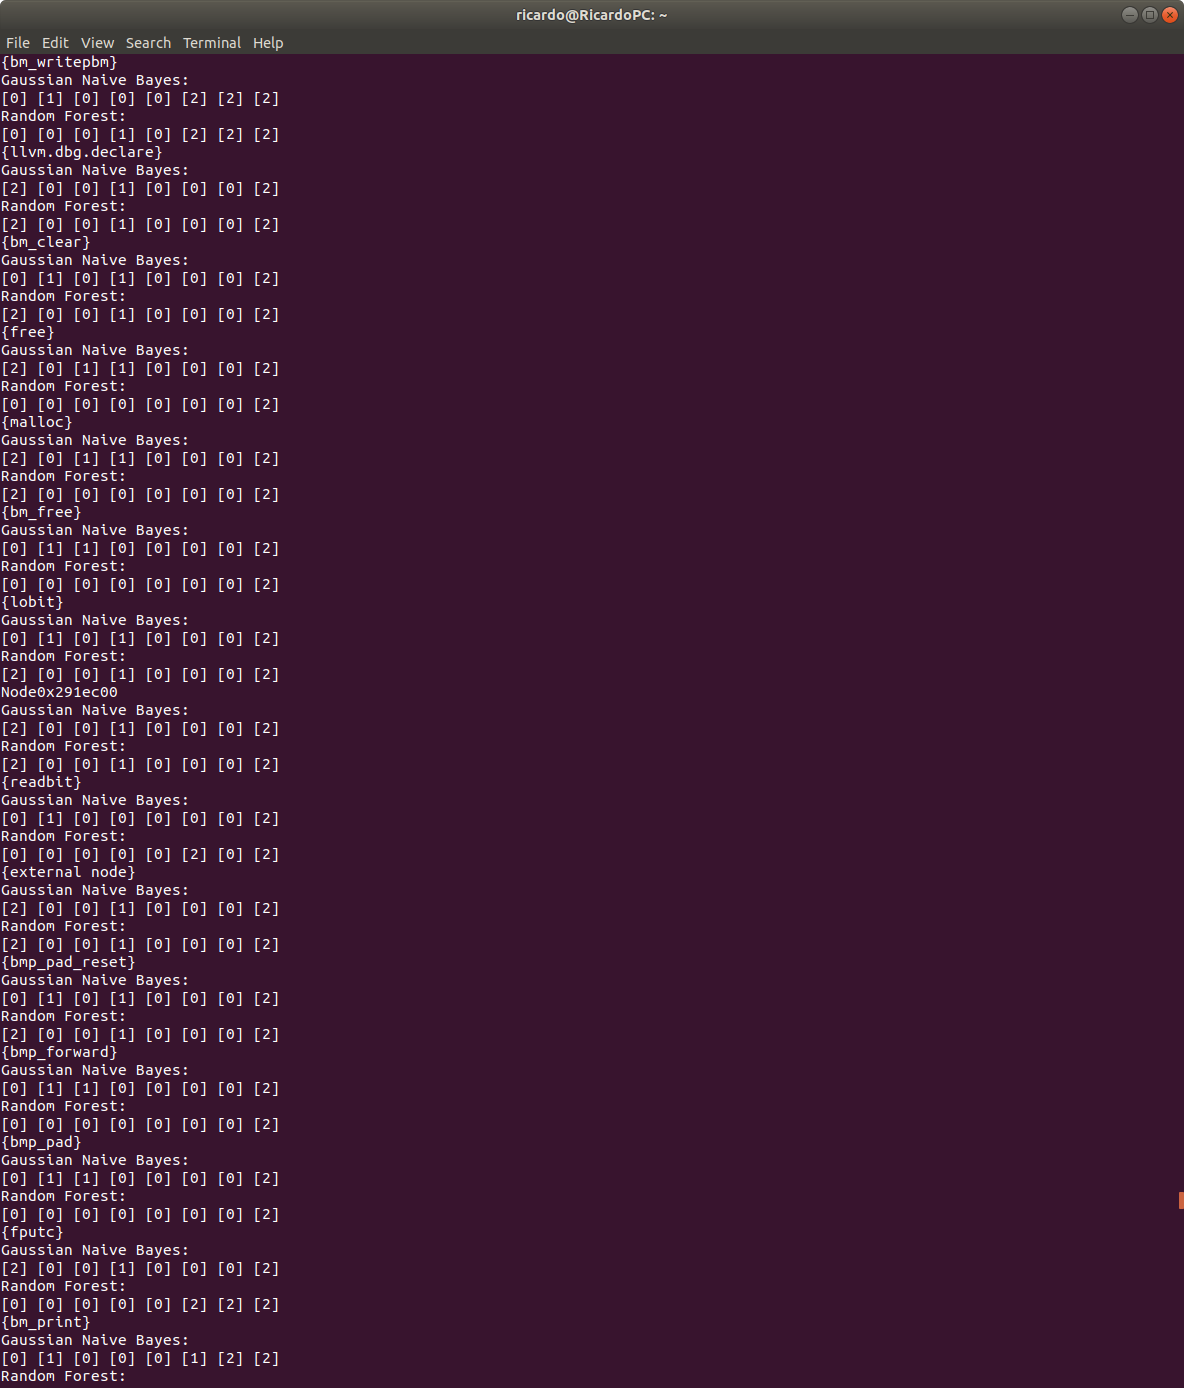
\includegraphics[width=0.7\textwidth]{vanilla_predictions}
\end{figure}

This was just a test of how these two classifiers would behave with the amount of data we were feeding into it. We did an accuracy test with both algorithms, using SciKit \parencite{scikit} simple cross-validation, without K-Folds.

\begin{table}[H]
	\centering
	\caption{Naive Bayes Accuracy Results}
	\begin{tabular}{ |p{4cm}||p{10cm}|  }
		\hline
		Base Metric Score & Accuracy\\
		\hline
		AV   & 0.54 (+/- 0.27) \\ 
		AC &   0.63 (+/- 0.22)  \\
		PR & 0.95 (+/- 0.07)  \\
		UI    & 0.55 (+/- 0.14)  \\
		S   & 0.89 (+/- 0.22)  \\
		C   & 0.65 (+/- 0.22)  \\
		I    & 0.65 (+/- 0.50)  \\
		\hline
	\end{tabular}
\end{table}

\begin{table}[H]
	\centering
	\caption{Random Forest Accuracy Results}
	\begin{tabular}{ |p{4cm}||p{10cm}|  }
		\hline
		Base Metric Score & Accuracy\\
		\hline
		AV   & 0.80 (+/- 0.08) \\ 
		AC &   0.97 (+/- 0.05)  \\
		PR & 1.00 (+/- 0.00)  \\
		UI    & 0.77 (+/- 0.08)  \\
		S   & 0.99 (+/- 0.05)  \\
		C   & 0.84 (+/- 0.17) \\
		I    & 0.81 (+/- 0.16)  \\
		\hline
	\end{tabular}
\end{table}

By taking a look we can clearly see that Random Forest is always better than its counterpart, and we attribute this largely to how good Random Forest handles smaller data sets, such as the one we have. After seeing the results, it became a simple decision and we decided to move on with Random Forest for the rest of the experimentation.

\subsubsection{All K-Fold Models}

In the next phase we would use K-Folds, as explained previously, in this case using a 4 fold, which would thereby provide 4 models, from which we will provide the results in the following tables:

\begin{table}[H]
	\centering
	\caption{First Model}
	\begin{tabular}{ |p{4cm}||p{10cm}|  }
		\hline
		Base Metric Score & Accuracy\\
		\hline
		AV   & 0.89 \\ 
		AC &   0.95  \\
		PR & 1.00  \\
		UI    & 0.95  \\
		S   & 1.00  \\
		C   & 0.84 \\
		I    & 0.89  \\
		\hline
	\end{tabular}
\end{table}

\begin{table}[H]
	\centering
	\caption{Second Model}
	\begin{tabular}{ |p{4cm}||p{10cm}|  }
		\hline
		Base Metric Score & Accuracy\\
		\hline
		AV   & 0.63 \\ 
		AC &   0.89  \\
		PR & 0.89  \\
		UI    & 0.79  \\
		S   & 0.79  \\
		C   & 0.84 \\
		I    & 0.84  \\
		\hline
	\end{tabular}
\end{table}

\begin{table}[H]
	\centering
	\caption{Third Model}
	\begin{tabular}{ |p{4cm}||p{10cm}|  }
		\hline
		Base Metric Score & Accuracy\\
		\hline
		AV   & 1.00 \\ 
		AC &   0.95  \\
		PR & 1.00  \\
		UI    & 1.00  \\
		S   & 1.00  \\
		C   & 0.95 \\
		I    & 0.95  \\
		\hline
	\end{tabular}
\end{table}

\begin{table}[H]
	\centering
	\caption{Fourth Model}
	\begin{tabular}{ |p{4cm}||p{10cm}|  }
		\hline
		Base Metric Score & Accuracy\\
		\hline
		AV   & 0.78 \\ 
		AC &   1.00  \\
		PR & 1.00  \\
		UI    & 0.83  \\
		S   & 1.00  \\
		C   & 0.78 \\
		I    & 0.78  \\
		\hline
	\end{tabular}
\end{table}

An interesting detail to note is that the AV (Attack Vector) had the lowest accuracy of all base scores, and way below the average, in our second model which leads us to believe that this base score could be improved upon with better impact factors in the future, since it is the "Attack Vector". We might be able to confirm if this was just an outlier case or if our model would be erratic once we had feedback from IT security professionals.

The rest performed around the average and there were no other outliers. We then proceeded to select our best model, with which we would predict all vulnerabilities found via compositional symbolic execution.

\subsubsection{Best model found}

By comparing all models, and storing only the ones with the best scores, we were able to come up with the following model:

\begin{table}[H]
	\centering
	\caption{Our Best and Final Model Found}
	\begin{tabular}{ |p{4cm}||p{10cm}|  }
		\hline
		Base Metric Score & Accuracy\\
		\hline
		AV   & 1.00 \\ 
		AC &   1.00  \\
		PR & 1.00  \\
		UI    & 1.00  \\
		S   & 1.00  \\
		C   & 0.95 \\
		I    & 0.95  \\
		\hline
	\end{tabular}
\end{table}

The results really exceeded our expectations, even though our dataset was small, the accuracy level was very high, but we are certain that this is not a coincidence and that the feedback from specialized professionals would reassure us that the impact factors selected were indeed indicators of how severe vulnerabilities are.

\subsection{Survey Results}

When we started our survey we expected our userbase to be IT security professionals who have experience with C or C++. As mentioned in the previous section, we asked for their opinion, and we encouraged them to leave their name, and e-mail so they could be contacted in case we wanted to request further feedback or to better our knowledge of details we might have overseen. We only provided the link to our tool to people that we knew met this criterion, mainly by directly contacting the developers of all the programs we used throughout this thesis so that we knew the people taking a look had enough experience and our data would not be noisy.

It is also worth noting that we tracked the following data:

\begin{itemize}
	\item Program that they had selected
	\item Functions they had analyzed
	\item Order in which said functions were selected
\end{itemize}

As well as the base scores they left selected -- in case they selected a vulnerable function -- at the time of the feedback's submission. The results were the following (We are not adding the names for privacy purposes):

\subsubsection{1st entry}

\begin{itemize}
	\item Program: jasper2
	\item Comment: Without pinpointing the vulnerable instruction, the function is very hard to analyze manually. 
	Looking at the size of this function (250 lines), it's might be a good idea to keep the score high, because it's likely to be reused somewhere. 
	I also think the signature of the function suggests the incoming parameters are very varied and, hence, might be prone to being unsanitized.  
	\item Selected Nodes: \{jpc\_dec\_decodepkt\}
\end{itemize}

\subsubsection{2nd entry}

\begin{itemize}
	\item Program: jasper2
	\item Comment: The tool looks great, but it would be really useful if for each function you would also indicate the number of the LOC where the buffer overflow vulnerability occurs. Otherwise, for large functions, it is difficult to pinpoint the vulnerability manually. Of course, it is also easier to analyze the code of commented functions in comparison to functions without any comments.
	\item Selected Nodes: \{jpc\_dec\_decodepkt\}\{external node\}\{jpc\_dec\_lookahead\}\{jpc\_dec\_decodepkts\}
\end{itemize}

\subsubsection{3rd entry}

\begin{itemize}
	\item Program: rzip
	\item Comment: All OK
	\item Selected Nodes: \{read\_buf\}\{write\_u16\}\{llvm.memcpy.p0i8.p0i8.i64\}\{BZ2\_bzBuffToBuffCompress\}\\\{write\_buf\}
\end{itemize}

\subsubsection{4th entry}

\begin{itemize}
	\item Program: rzip
	\item Comment: All is OK but for this file I'm not sure the result of confidentiality
	\item Selected Nodes: \{read\_buf\}\{write\_u16\}\{llvm.memcpy.p0i8.p0i8.i64\}\{BZ2\_bzBuffToBuffCompress\}\\\{write\_buf\}\{read\_u8\}
\end{itemize}

\subsubsection{5th entry}

\begin{itemize}
	\item Program: rzip
	\item Comment: Agree with this calculation.
	\item Selected Nodes: \{read\_buf\}\{write\_u16\}\{llvm.memcpy.p0i8.p0i8.i64\}\{BZ2\_bzBuffToBuffCompress\}\\\{write\_buf\}\{read\_u8\}\{read\_stream\}
\end{itemize}

\subsubsection{6th entry}

\begin{itemize}
	\item Program: rzip
	\item Comment: I think the file is use locally.
	\item Selected Nodes: \{read\_buf\}\{write\_u16\}\{llvm.memcpy.p0i8.p0i8.i64\}\{BZ2\_bzBuffToBuffCompress\}\\\{write\_buf\}\{read\_u8\}\{read\_stream\}\{write\_stream\}\{write\_u32\}
	
\end{itemize}

\subsubsection{Take away from the survey}

We think that there are two main key points to take away from this: First, our framework had a good user interface, which received praise for its look and feel, though at the same time received criticism for the lack of features, which would take time away from the assessment of vulnerabilities, which ultimately is our goal. Second, our model's accuracy has been confirmed to some extent by professionals, but the amount of data is not enough to draw a solid conclusion.

What we can say from the professionals' comments is that our predictions are on the right track, and perhaps one base score might be out of place. There is also the subjectivity factor, which can be seen by looking at the feedback, and how some developers thought the prediction was spot-on and some thought it needed a bit of polish. In the end, we can certainly say that the cross-validation scores were not an anomaly and that the impact factors were correct when assessing vulnerabilities and using CVSS as the metric to do so.
